\chapter{Desarrollo: Iteración III} % Main chapter title

\label{Chapter8} % Change X to a consecutive number; for referencing this chapter elsewhere, use \ref{ChapterX}

\steveCabecera{Capítulo 8. \emph{Iteración III}} % Change X to a consecutive number; this is for the header on each page - perhaps a shortened title

%----------------------------------------------------------------------------------------
%	SECTION 1
%----------------------------------------------------------------------------------------
\section{Introducción}
En este capítulo se documentan aspectos relevantes relacionados con la codificación que se realizó en la tercera iteración de desarrollo del software.\\
Aparece un nuevo requerimiento funcional a partir de la devolución de un grupo de early testers quienes solicitaron un modo de accionamiento rápido a través de alguna interfaz en la pantalla de bloqueo de android.
Quizás el cambio más importante introducido en esta iteración es la inclusión del canal de comunicación con los módulos a través de internet. Se describirá el modo de empleo del protocolo MQTT para conseguir la ejecución de los RPC. Se codificó un wrapper reactivo sobre la librería paho de eclipse empleada para configurar el cliente MQTT y su posterior empleo en la aplicación. %%Request Response over Subscribe Queues, message duplicaction,message payload format
Dado que se habilitó un nuevo canal, el repositorio deberá decidir cuando ejecutar los RPC por LAN o Internet, se expondrá el algoritmo utilizado para la selección de los canales.
Finalmente así como se hizo para las iteraciones previas se expondrán las implementaciones más interesantes de la lógica de negocios de los caso de uso planificados para esta iteración.
%% implementaion sofisticada con templates genericos
\section{Accionamiento Rápido}
Luego de producir las primeras unidades del módulo
decidimos distribuirlas a un grupo de usuarios que estaban interesados en probar el producto.
Pasado el período de pruebas nos pusimos en contacto con ellos y tomamos registro de sus devoluciones.
Un comentario común entre la mayoría fue que les parecía que tenían que hacer demasiado para accionar sus portones.
Apareció entonces la propuesta de adicionar un elemento visual en la pantalla de bloqueo de android
que permita el accionamiento sin tener que desbloquear el teléfono.

En la figura ~\ref{fig:notif_design} se puede ver una maqueta de cómo luciría el control rápido implementado como una notificación permanente de android.

Como medidas de seguridad para evitar accionamientos accidentales se propuso limitar los módulos
disponibles para este tipo de accionamiento a aquellos que se encuentren dentro de un radio de 320 metros alrededor del teléfono. También se incluyó un segundo botón que habilita el accionado, obligando al usuario a realizar 2 movimientos voluntarios para completar la acción: tomando como referencia la figura ~\ref{fig:notif_design} será necesario presionar el botón (3) y luego el botón (4).


\begin{figure}[htbp]
	\centering
	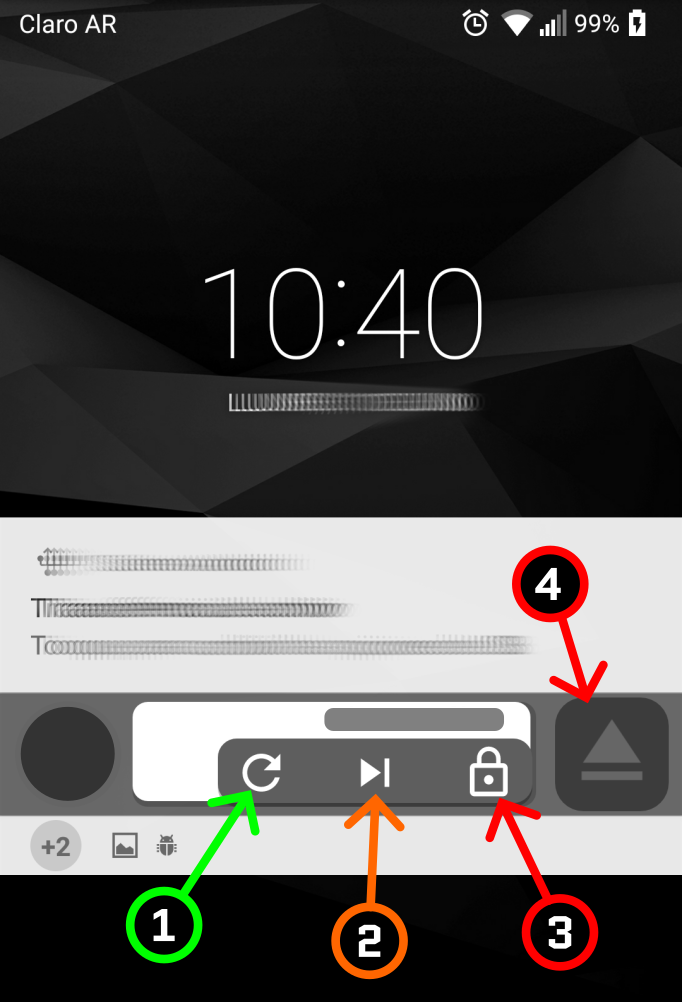
\includegraphics[width=0.4\textwidth]{Figures/iter3/module_notif.png}
	\rule{35em}{1pt}
	\caption[Wireframe]{Esquema de diseño de la notificación permanente para el control rápido. (1) Boton para buscar los módulos disponibles, (2) Boton para rotar el módulo seleccionado, (3) Botón para habilitar el accionamiento, (4) Botón para accionar el módulo seleccionado.}
	\label{fig:notif_design}
\end{figure}

\section{Canal de comunicación por Internet}
Uno de los aspectos más sobresalientes de la propuesta de valor del producto es la posibilidad
de monitorear, configurar y accionar el módulo de manera remota a través de internet.
El modo de conexión completo se puede observar en la figura ~\ref{lebxx} 
\subsection{Adaptación del protocolo MQTT}
Como se mencionó en la sección ~\ref{section:xxx} el protocolo MQTT implementa el patrón de arquitectura Publish-Subscribe
sin embargo está claro que la ejecución de protocolos RPC necesita de un canal de comunicación que admita  Request-Response...
Esta controversia se resuelve del lado de la aplicación ofreciendo una adaptación sobre el protocolo MQTT.
Es decir, la suscripción a los tópicos, el envío de mensajes y el formato de los mismos se realizará de manera tal que el modo de comunicación entre aplicación y módulos Request-Response.
\subsubsection{Formato del Mensaje}

\subsubsection{Esquema de Suscripciones}

\subsection{RPC sobre MQTT}

\subsection{Selector de Canales}

\subsubsection{Ejecutor}


\section{Casos de Uso Implementados}
Para la presente iteración se implementaron los siguientes casos de uso.
\begin{enumerate}
	\item Actualizar GATE-STATUS de los módulos.
	\item Activar Acceso Rápido.
	\item Actualizar Firmware
	\item Habilitar Módulo para Acceso Rápido.
	\item Accionar módulo cercano.
	\item Obtener módulos disponibles para acceso rápido.
	\item Desbloquear botón contra accionamiento accidental.
\end{enumerate}

A continuación se documentaran aquellos que presentan los escenarios más interesantes.

\subsection{Actualizar Firmware}
Este caso de uso es fundamental para garantizar la calidad del producto al proveer actualizaciones para el firmware del módulo.
El usuario administrador ingresa a la pantalla de configuración de un módulo, luego toca el botón asignado para esta operación, acepta el cartel de advertencia y espera hasta que concluya el procedimiento.
Como una nota al margen se menciona que por restricciones impuestas en el framework utilizado para programar el firmware del módulo la actualización OTA solo puede realizarse por el canal LAN y consiste de los siguientes pasos:
\begin{enumerate}
	\item El teléfono descarga un archivo .zip que corresponde a la nueva versión del firmware para el módulo.
	\item El teléfono envía este archivo al módulo mediante un POST HTTP multiparte a un endpoint predefinido que incluye el archivo del nuevo firmware y el valor \texttt{COMMIT\_TIMEOUT} que determina la cantidad de tiempo en segundos que esperará el módulo para que el usuario autorice la nueva versión luego de concluida la instalación y el reinicio exitoso.
	\item El teléfono espera que el módulo se reinicie y ejecuta el RPC GetSysInfo para corroborar la correcta versión del firmware recién instalado.
	\item COMMIT: El teléfono hace un POST HTTP a un endpoint predefinido para autorizar la actualización.
\end{enumerate} 

Este caso de uso utiliza hasta tres RPC en su ejecución y puede fallar en 8 escenarios distintos a saber:

\begin{enumerate}
	\item Error de comunicación con el módulo.
	\item Versión actual del firmware DESCONOCIDA.
	\item Actualización no necesaria.
	\item Error con la URL de descarga del archivo de firmware.
	\item El archivo descargado está vacío.
	\item Error de comunicación con el servidor.
	\item Error de versión después de actualizar.
	\item Error de COMMIT.
\end{enumerate} 

En el diagrama de la figura ~\ref{fig:act_ota} se puede observar el algoritmo implementado para este caso de uso.

\begin{figure}[htbp]
	\centering
	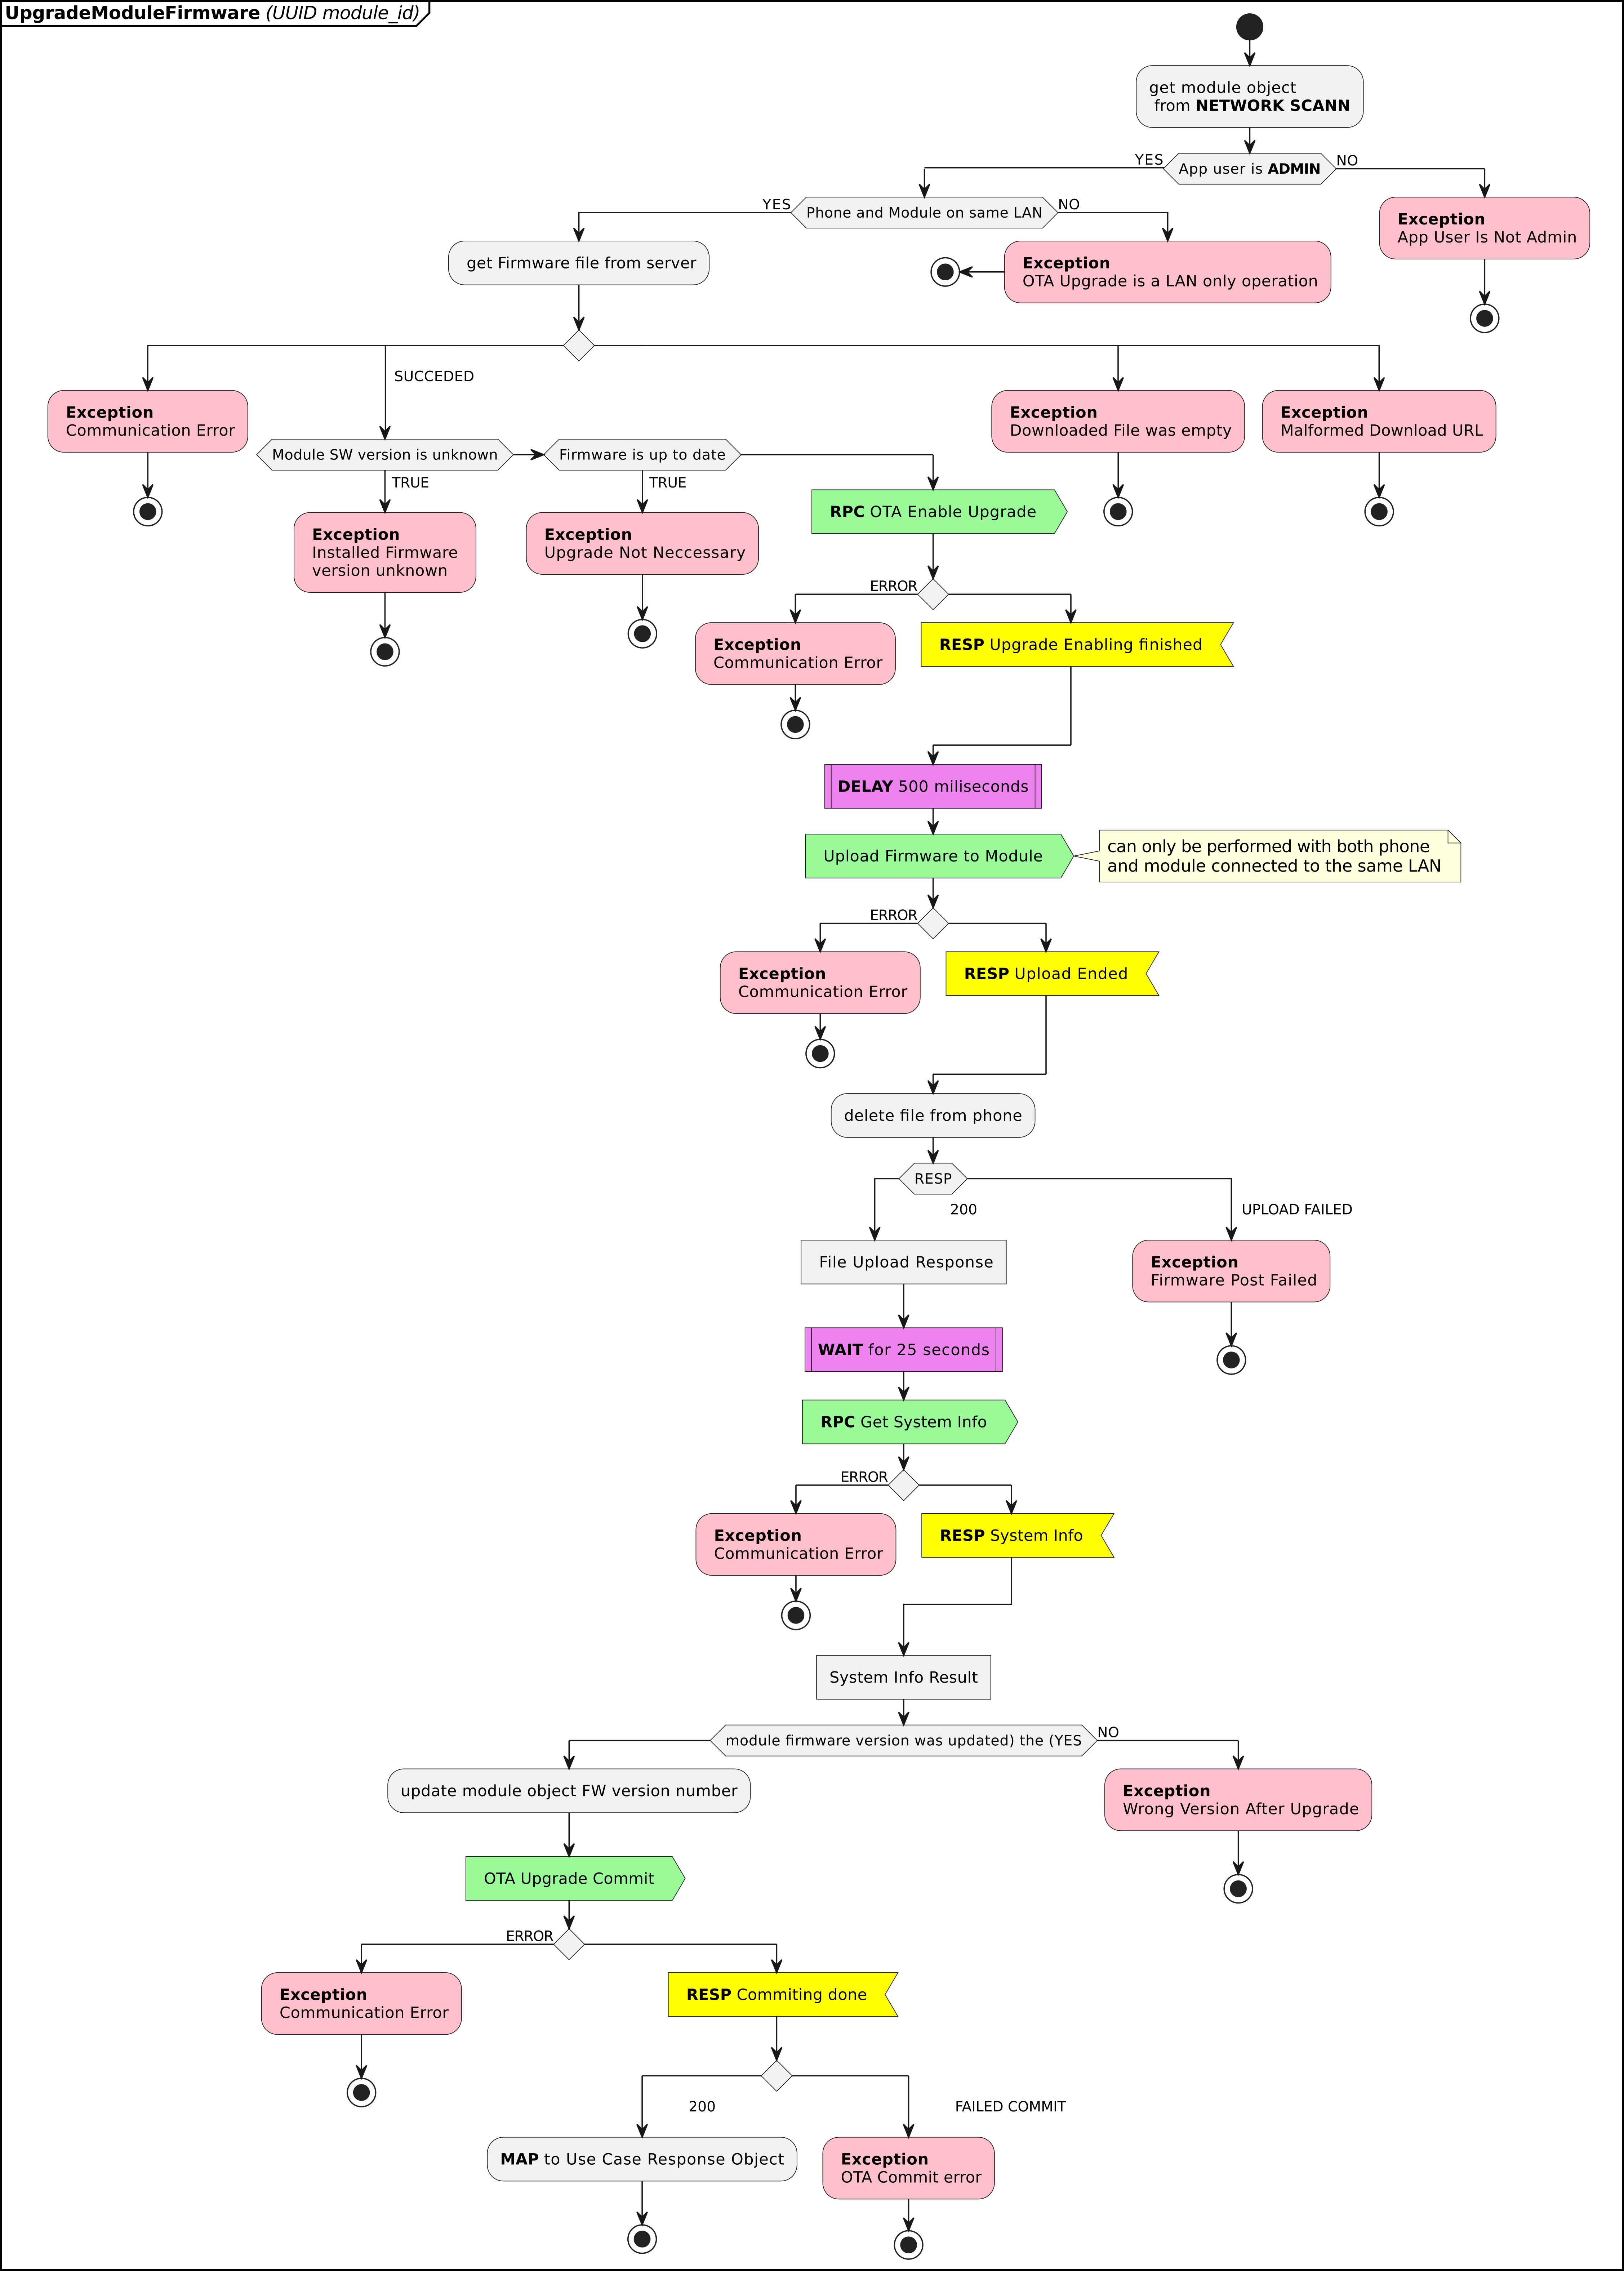
\includegraphics[width=\textwidth]{Figures/iter3/ACT_ota_ink.png}
	\rule{35em}{1pt}
	\caption[Class Diagram]{Diagrama de actividades de la implementación del caso de uso: Actualización de Firmware.}
	\label{fig:act_ota}
\end{figure}

\subsection{Obtener módulos disponibles para acceso rápido}
En la pantalla de bloqueo del teléfono sobre la notificación permanente el usuario presiona
el botón para refrescar los módulos disponibles para accionamiento rápido.
Este caso de uso obtiene la ubicación geográfica del teléfono que debe tener una precisión menor a 60 metros
y su última actualización no debe superar los 5 minutos.
Una vez conocida la posición geográfica del teléfono buscará todos los módulos que cumplan las siguientes condiciones:
\begin{itemize}
	\item El modulo debe estar en STATION\_MODE.
	\item El usuario de la app debe estar autorizado.
	\item El modulo debe tener habilitado el control rápido.
	\item El módulo debe encontrarse a menos de 320 metros de distancia.
\end{itemize}
Este caso de uso no realiza llamadas a RPCs y puede fallar en 8 escenarios.
En la figura ~\ref{fig:act_notif_modules} se puede observar el diagrama de actividades de la implementación del caso de uso.

\begin{figure}[htbp]
	\centering
	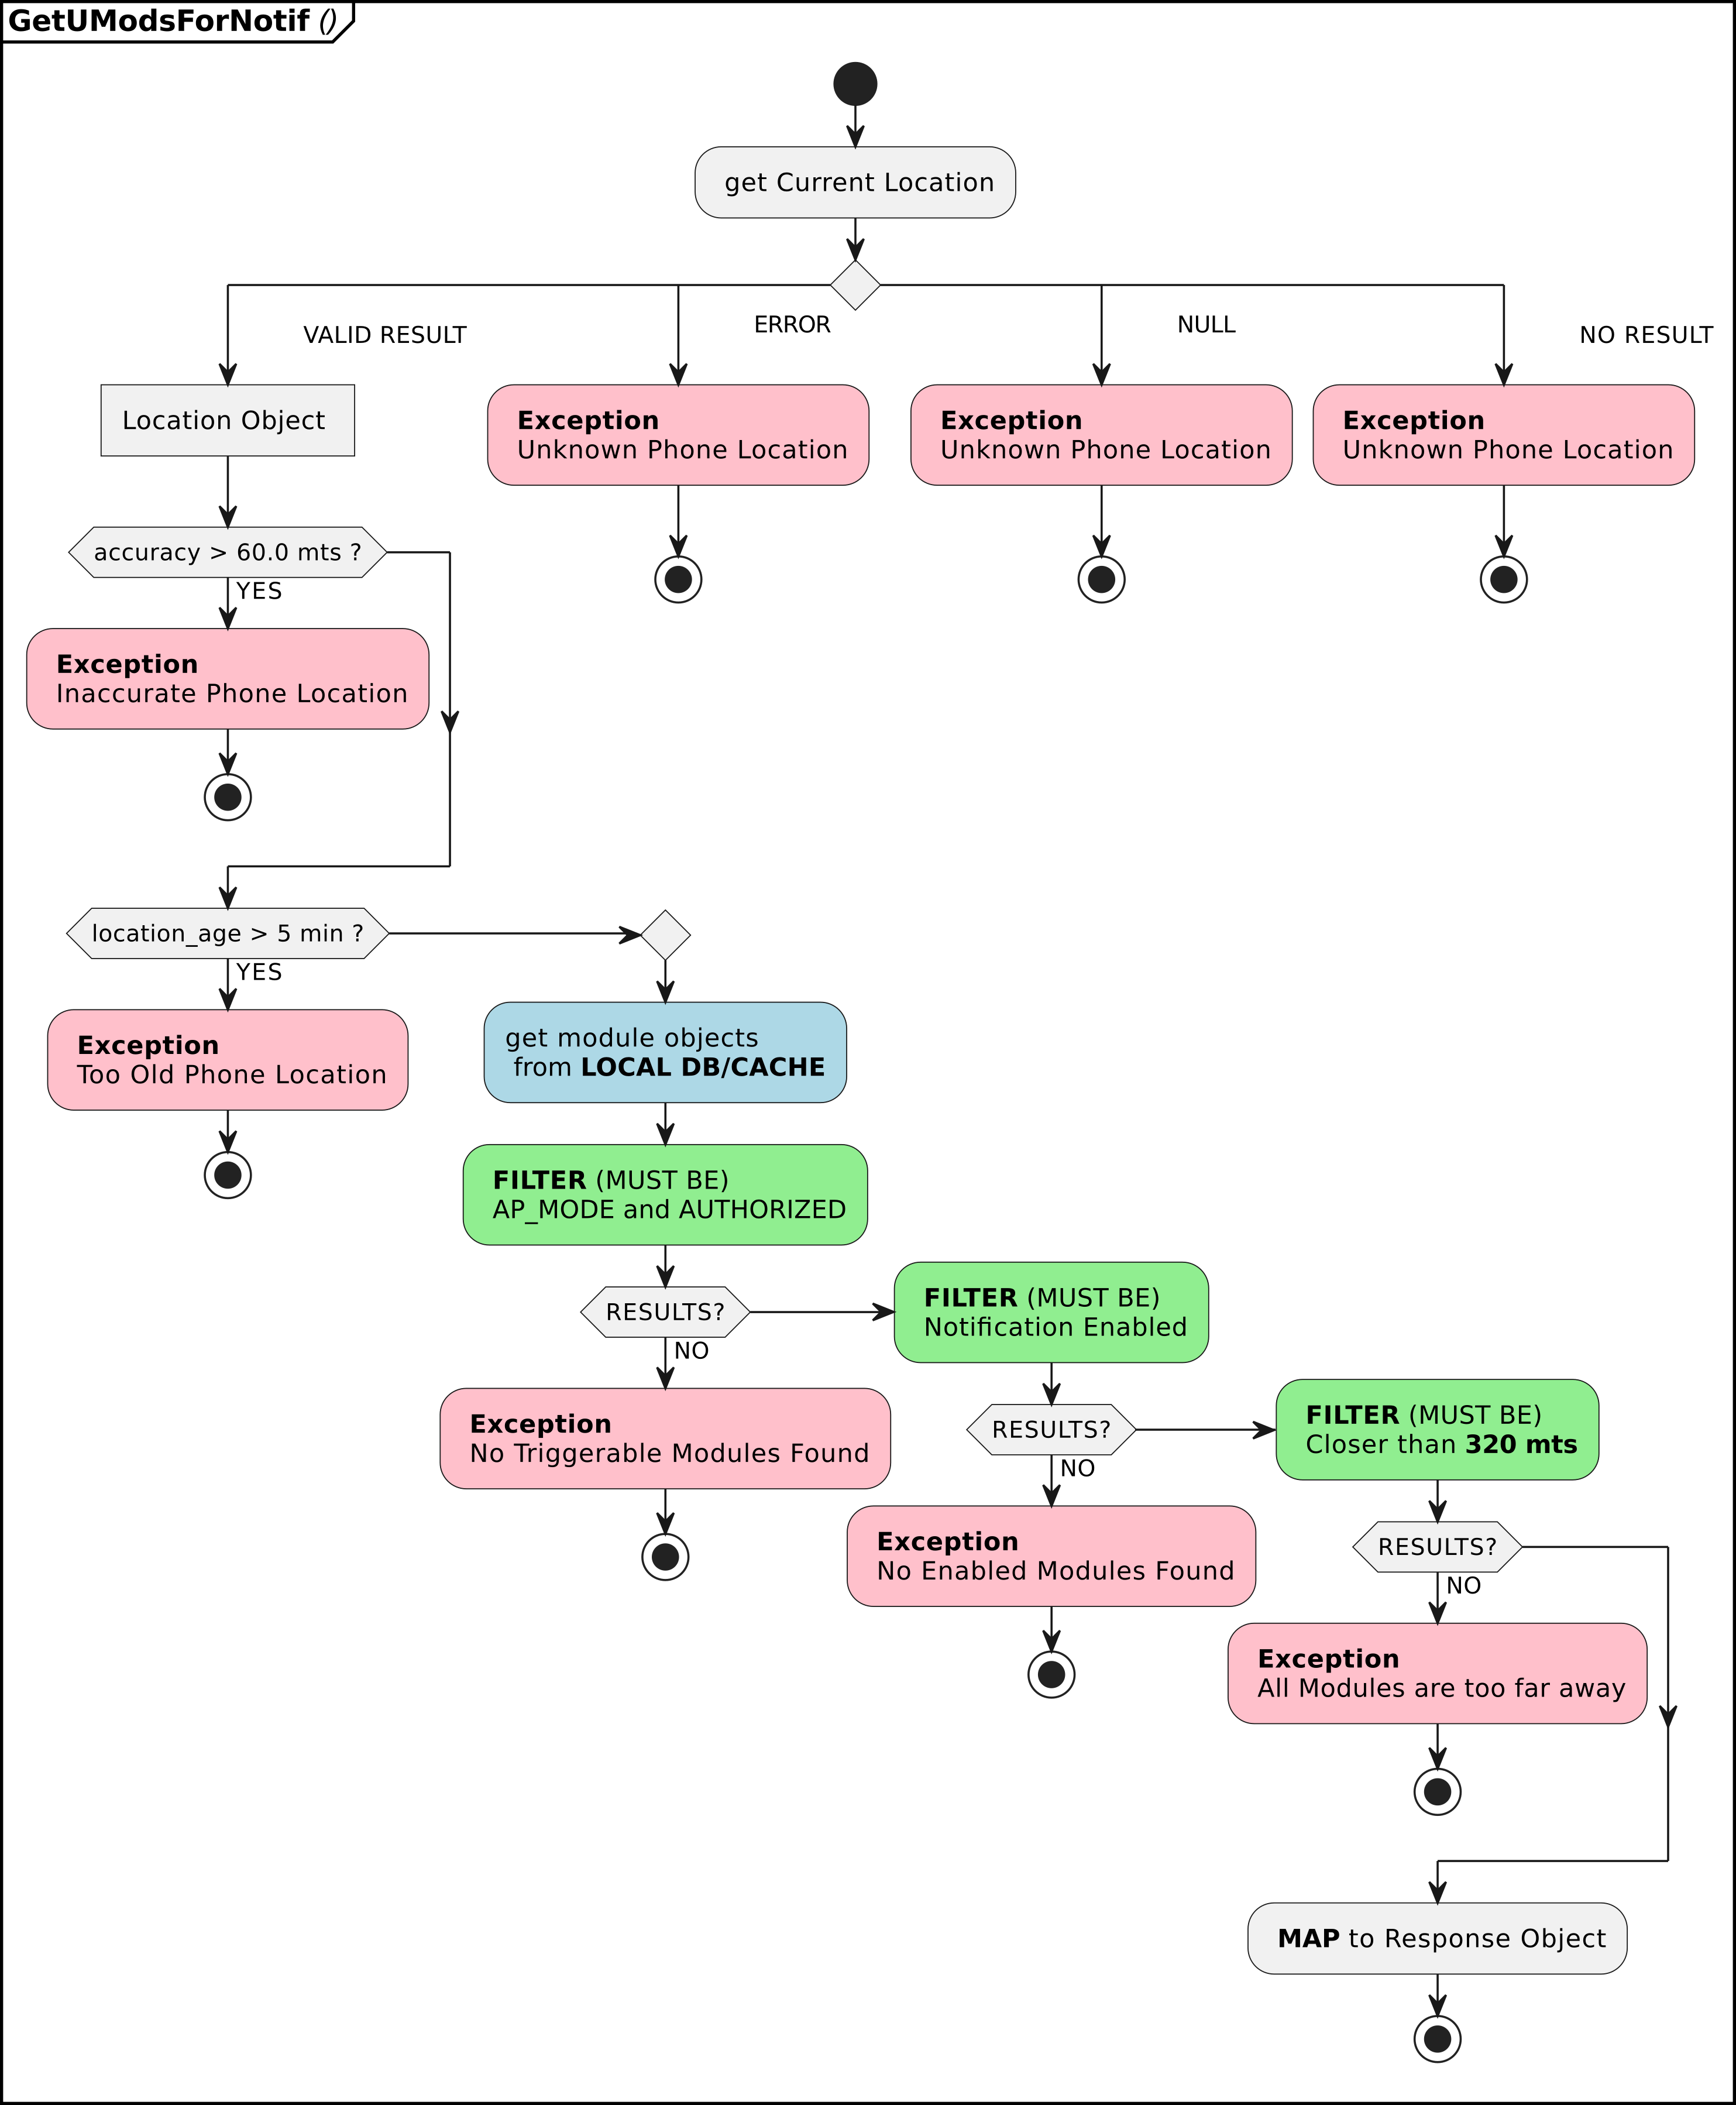
\includegraphics[width=0.8\textwidth]{Figures/iter3/ACT_getModsNotif.png}
	\rule{35em}{1pt}
	\caption[Class Diagram]{Diagrama de actividades de la implementación del caso de uso: Obtener módulos disponibles para acceso rápido.}
	\label{fig:act_notif_modules}
\end{figure}

